\subsection{The Halved Model}

The idea behind the halved model is that the model we have can be looked at in a different way than it was introduced in.
We know the model maps an input $x$ to $f(x) \mod 1$, meaning that if the output $f(x)$ is greater or equal to 1, we subtract 1 from it until it is in the range $[0, 1)$.
Similarly, we add 1 to it if it is smaller than 0 until it is in the desired range.
Now instead of confining the model to the domain of $[0, 1)$, we think of it repeating infinitely in both directions.
We can achieve this by mapping $x$ to $f(x - \lfloor x \rfloor)$.
This trick maps the input $x$ into the domain, on which our model function produces sensible results and causes it to repeat infinitely.
\Cref{fig:minrep.infinite.model.concept} illustrates this concept for the cycle $P_7^3$.
The blue square is the full model.
One can see, that the branch $f_\D$ is outside the blue square at its right edge.
This is because it was cut off and continued at the bottom of the square before, due to the $\mod 1$ operation.

\todo{this makes sense in the original problem domain}

In this model, there are no cycles that have multiple rotations.
Instead, the cycles that had multiple rotations in the full model, manifest as a sequence of different blocks of the full model.
Meaning for the example $P_7^3$, the same blocks of $\A^4\B^3\C^4\D^3$ are repeating infinitely.
But for an example with multiple rotations, such as $\A\B\C\D\A^2\B^2\C^2\D^2$, the blocks will not all be the same.
Instead, the blocks $\A\B\C\D$ and $\A^2\B^2\C^2\D^2$ will be alternating.

Now the symmetry of our function $f$ comes into play.
Since $f(x + 0.5) = f(x) + 0.5$ for $x \in [0, 0.5)$, we can split the infinite model into smaller blocks than the blue block of the full model.
The function of the infinite model repeats in blocks of size 0.5, these blocks are marked red in \Cref{fig:minrep.infinite.model.concept}.
These red blocks represent the halved model, it is the smallest repeating part of the infinite model.
To get the cycle in the halved model, we look at the pattern in which different red blocks repeat along the infinite model.
For our example in the picture, there is only one red block that repeats infinitely, $\L^4\R^3$.
The next section will explain, how to translate cycles between the halved and full model.

\begin{figure}
	\centering
	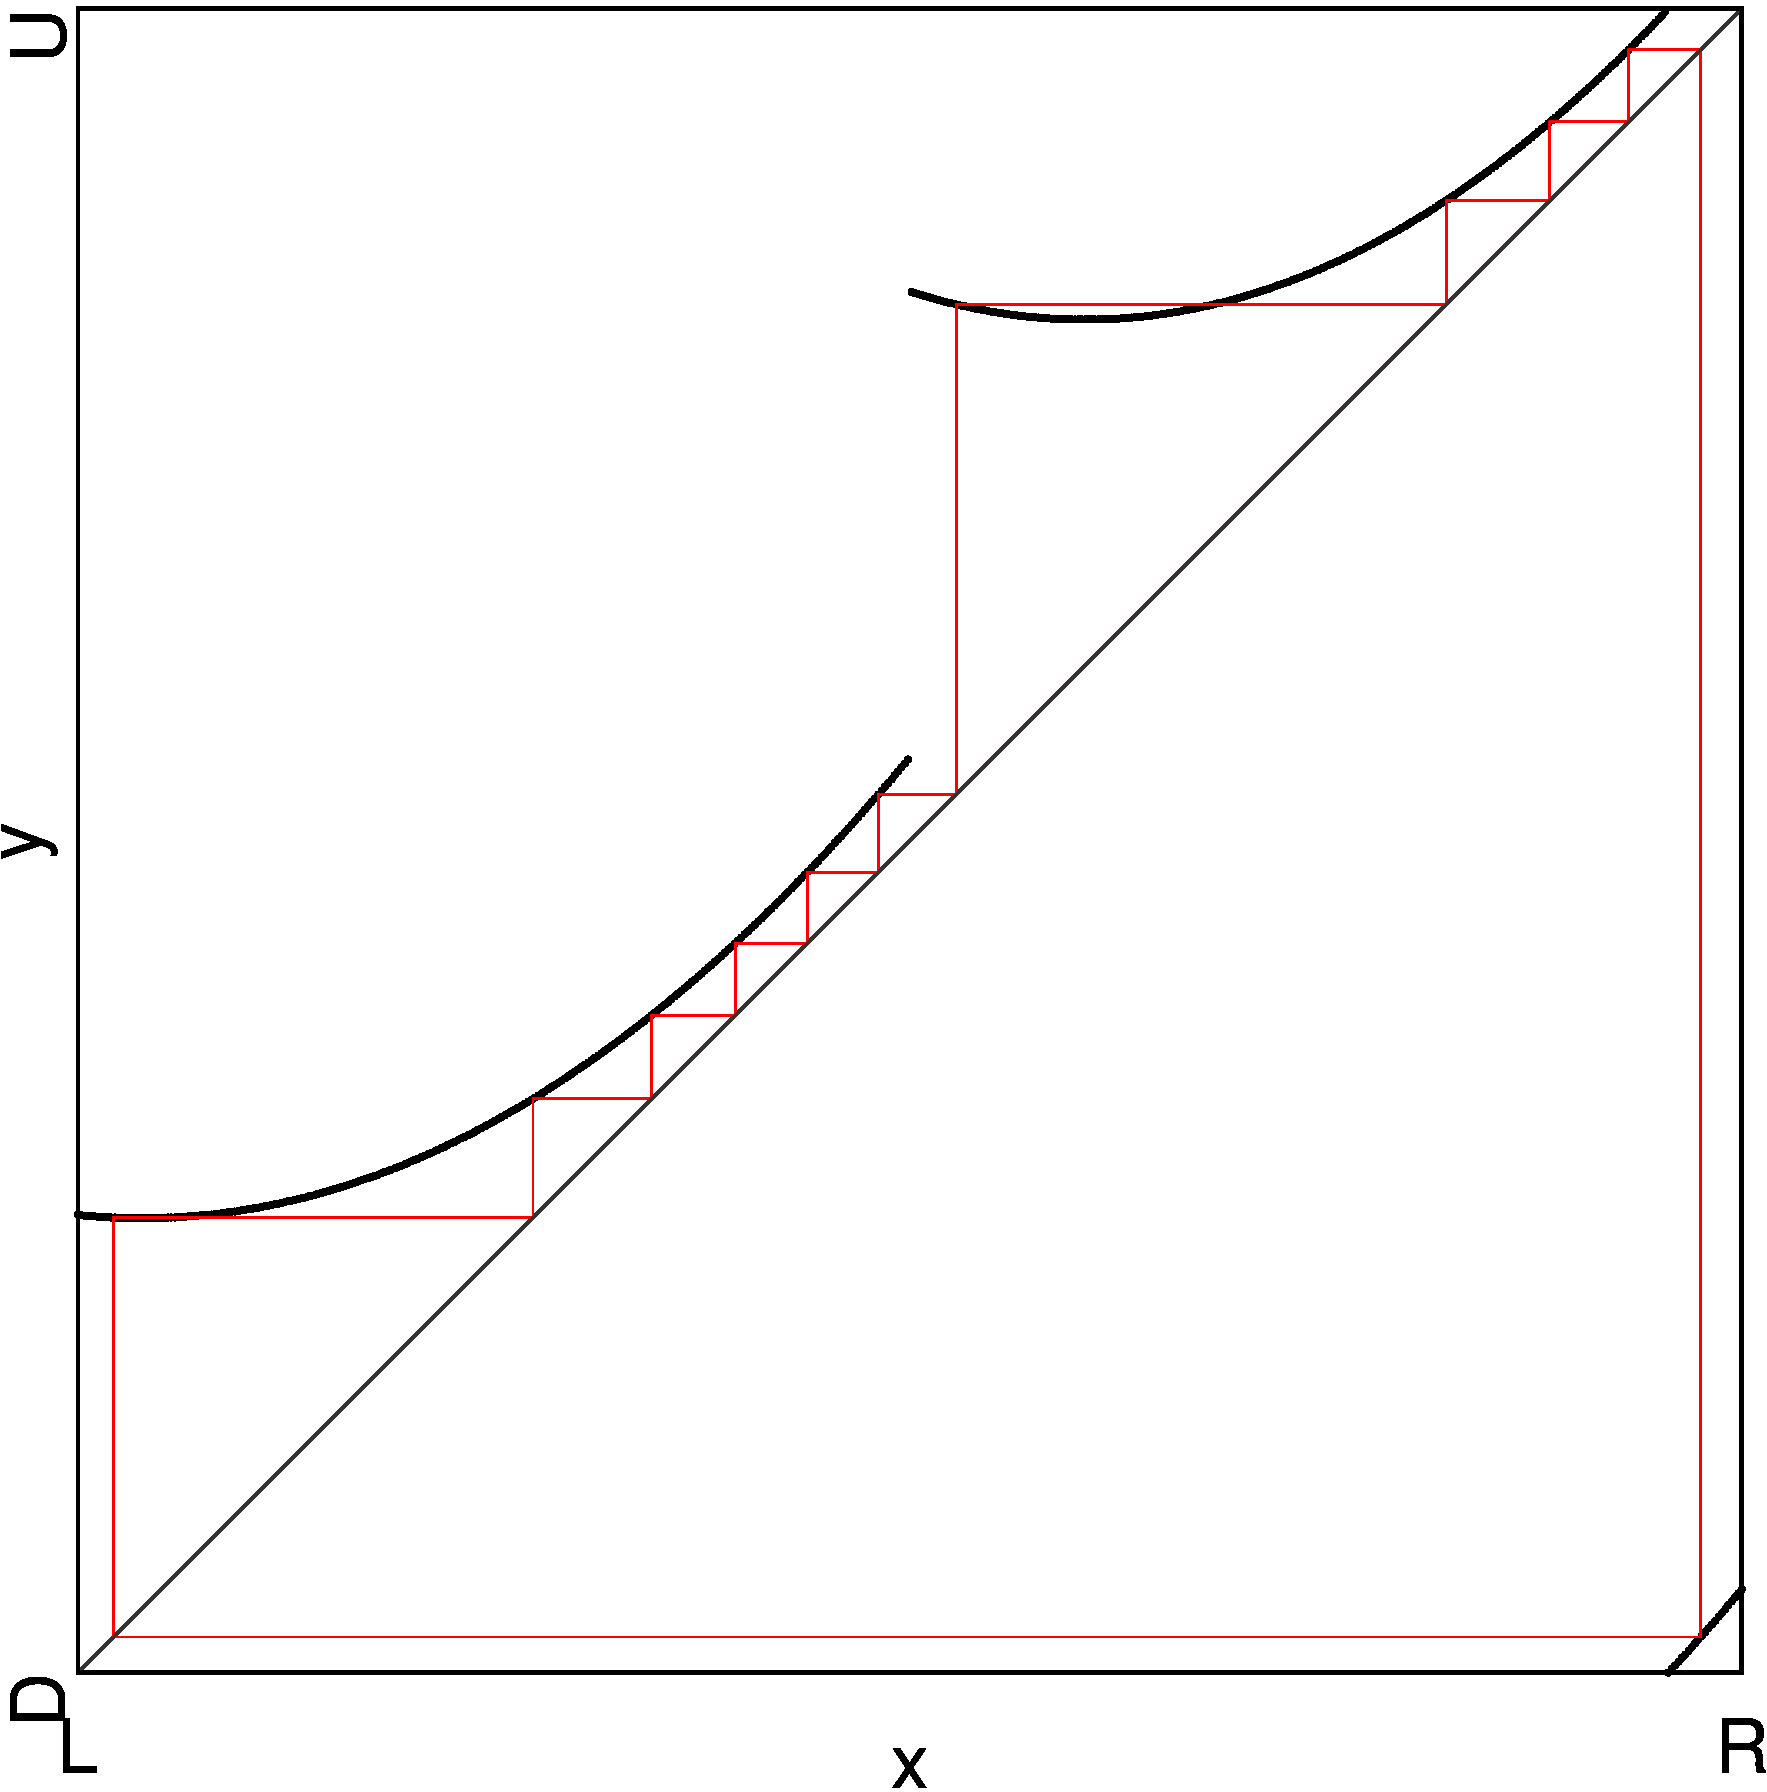
\includegraphics[width=.7 \textwidth]{63_MinimalRepr_Adding_Halved/Cob_Vis_s/Manual/result.png}
	\caption{Illustration of the infinite model concept.}
	\label{fig:minrep.infinite.model.concept}
\end{figure}

\subsubsection{Naive Algorithm}

\todo{rewrite naive algo to use introduction as basis}
\todo{start with f -> halved since it was teased at the end of the last section}

We start with a naive algorithm for translating a cycle from the halved model to the full model.
This process will be called ``unrolling'' since you fit two rotations in the halved model into one rotation in the full model.
\todo{Visualize unrolling}

The input is a cycle in the halved model, $h = \L^{l_1}\R^{r_1}\L^{l_2}\R^{r_2} \ldots \L^{l_n}\R^{r_n}$.
First, we write down the input cycle twice.
\begin{align}
	h|h & = \L^{l_1}\R^{r_1}\L^{l_2}\R^{r_2} \ldots \L^{l_n}\R^{r_n} | \L^{l_1}\R^{r_1} \ldots \L^{l_n}\R^{r_n}
\end{align}
Then we pair up the rotations.
We need to write the original cycle twice because we will translate two rotations in the halved model to one rotation in the full model.
If we were to write it down only once and the number of rotations $n$ happens to be odd, the rotation $\L^{l_n}\R^{r_n}$ would be left over.
To make it work out, we need to continue pairing up the cycles, wrapping around, or equivalently writing down the original cycle twice.
After we paired up the rotations, we translate the pairs of rotations with the function $t: \L^a\R^b\L^c\R^d \mapsto \A^a\B^b\C^c\D^d$.
\todo{Put in definition? Then $r$ and $r'$ should get a definition block too}
\begin{subequations}
	\begin{align}
		T(h) & = t(\L^{l_1}\R^{r_1}\L^{l_2}\R^{r_2}) \dots t(\L^{l_{n-1}}\R^{r_{n-1}}\L^{l_n}\R^{r_n}) \\
		     & = \A^{l_1}\B^{r_1}\C^{l_2}\D^{r_2} \dots \A^{l_{n-1}}\B^{r_{n-1}}\C^{l_n}\D^{r_n}
	\end{align}
\end{subequations}

Now that we got one cycle in the full model, we need to repeat the pairing and translating with every rotation as the starting point.
For this, we just rotate the cycle $h|h$ once with the function $r: \tau_1\tau_2 \dots \tau_n \mapsto \tau_2 \dots \tau_n\tau_1$, where $\tau$ is one rotation in the halved model.
\begin{align}
	r(h|h) & = \L^{l_2}\R^{r_2} \ldots \L^{l_n}\R^{r_n} | \L^{l_1}\R^{r_1} \ldots \L^{l_n}\R^{r_n} | \L^{l_1}\R^{r_1}
\end{align}
After pairing the rotations and translating the pairs with $t$, we get
\begin{subequations}
	\begin{align}
		T(r(h)) & = t(\L^{l_2}\R^{r_2}\L^{l_3}\R^{r_3}) \dots t(\L^{l_{n}}\R^{r_{n}}\L^{l_1}\R^{r_1}) \\
		        & = \A^{l_2}\B^{r_2}\C^{l_3}\D^{r_3} \dots \A^{l_{n}}\B^{r_{n}}\C^{l_1}\D^{r_1}
	\end{align}
\end{subequations}

We repeat this with $r^2$, $r^3$, and so on until $r^{n-1}$.
The resulting cycles may be equivalent by rotating in the full model.
We are only interested in the inequivalent cycles, these are the manifestations of the input cycle in the full model.

\begin{definition}
	Two cycles in the full model are equivalent $f_1 \equiv f_2$ if the cycles have the same number of rotations $n$ and there exists an integer $0 \leq i < n$ so that $r'^i(f_2) = f_1$.
	Where $r': \tau'_1\tau'_2 \dots \tau'_n \mapsto \tau'_2 \dots \tau'_n\tau'_1$ is the act of rotating a cycle in the full model and $\tau'$ is one rotation in the full model.
	Or there is an integer $j$, such that $f_1^j = f_2$ or $f_1 = f_2^j$.
\end{definition}

\begin{lemma}
	The translations of the two cycles $h_1$ and $h_2 = r^{2i}(h_1)$ in the halved model are equivalent $T(h_1) \equiv T(h_2)$ for all integers $i$.
\end{lemma}

\begin{proof}
	Let $h_1 = \tau_1\tau_2 \dots \tau_n$, therefore $h_2 = \tau_{2i+1} \dots \tau_n\tau_1 \dots \tau_{2i}$.
	The translations are $T(h_1) = t(\tau_1\tau_2)t(\tau_3\tau_4) \dots t(\tau_{n-1}\tau_n)$
	and $T(h_2) = t(\tau_{2i+1}\tau_{2i+2}) \dots t(\tau_{n-1}\tau_n)t(\tau_1\tau_2) \dots t(\tau_{2i-i}\tau_{2i})$.
	We can see that $T(h_2) = r'^i(T(h_1))$ and therefore $T(h_1) \equiv T(h_2)$.
\end{proof}

Therefore, we don't have to look at all rotations as a starting point for pairing, as described above.
It is enough to check both $T(h)$ and the once rotated case $T(r(h))$.
Therefore, each cycle in the halved model has at most 2 manifestations in the full model.

\subsubsection{Connections}
\todo{Better title}

\begin{theorem}
	A cycle in the halved model manifests either as a single cycle or two coexisting cycles in the full model.
\end{theorem}

\begin{theorem}
	\begin{enumerate}
		\item In the case of two coexisting cycles in the full model, the period of either cycle is half of the period of the cycle in the halved model: $|T(h)| = |T(r(h))| = \frac{1}{2} |h|$.
		\item In the case of one cycle in the full model, the period of this cycle is the same as the period of the cycle in the halved model: $|T(h)| = |T(r(h))| = |h|$.
	\end{enumerate}
\end{theorem}

\begin{theorem}
	\label{theorem:coex.even.odd}
	\begin{enumerate}
		\item The cycle $h$ manifests as two coexisting cycles in the full model, if and only if its number of rotations $n$ is even.
		\item The cycle $h$ manifests as one single cycle in the full model, if and only if its number of rotations $n$ is odd.
	\end{enumerate}
\end{theorem}

\begin{proof}
	\begin{enumerate}
		\item Let the number of rotations $n$ of $h$ be even
		      \begin{enumerate}[label=\alph*)]
			      \item Not rotated
			            \begin{align*}
				            T(h) & = t(\tau_1\tau_2) \dots t(\tau_{n-1}\tau_n) t(\tau_1\tau_2) \dots t(\tau_{n-1}\tau_n) \\
				                 & = (t(\tau_1\tau_2) \dots t(\tau_{n-1}\tau_n))^2                                       \\
				                 & \equiv t(\tau_1\tau_2) \dots t(\tau_{n-1}\tau_n) = a
			            \end{align*}
			      \item Rotated once
			            \begin{align*}
				            T(r(h)) & = t(\tau_2\tau_3) \dots t(\tau_{n}\tau_1) t(\tau_2\tau_3) \dots t(\tau_{n}\tau_1) \\
				                    & = (t(\tau_2\tau_3) \dots t(\tau_{n}\tau_1))^2                                     \\
				                    & \equiv t(\tau_2\tau_3) \dots t(\tau_{n}\tau_1) = b
			            \end{align*}
		      \end{enumerate}
		      We can see that $a \nequiv b$, unless $\tau_1 = \tau_2 = \tau_3 = \dots = \tau_n$.
		      For our adding structures, there must exist two integers $i, j$, for which $\tau_i \neq \tau_j$.
		      Also, we can see that the periods of the translated cycles are the same as the period of the original cycle.
		      The function $t$ preserves the period of the cycle, so $|\L^a\R^b\L^c\R^d| = a + b + c + d = |t(\L^a\R^b\L^c\R^d)| = |\A^a\B^b\C^c\D^d|$.
		      \begin{align*}
			      |a| & = |t(\tau_1\tau_2) \dots t(\tau_{n-1}\tau_n)|                                                       \\
			          & = \frac{1}{2} |(t(\tau_1\tau_2) \dots t(\tau_{n-1}\tau_n))^2|                                       \\
			          & = \frac{1}{2} |t(\tau_1\tau_2) \dots t(\tau_{n-1}\tau_n) t(\tau_1\tau_2) \dots t(\tau_{n-1}\tau_n)| \\
			          & = \frac{1}{2} |\tau_1\tau_2 \dots \tau_n\tau_1 \dots \tau_n|                                        \\
			          & = |\tau_1\tau_2 \dots \tau_n| = |h|
		      \end{align*}
		      Analogously for $|b| = |h|$.
		\item Let the number of rotations $n$ of $h$ be odd
		      \begin{enumerate}[label=\alph*)]
			      \item Not rotated
			            \begin{align*}
				            T(h) & = t(\tau_1\tau_2) \dots t(\tau_{n}\tau_1) t(\tau_2\tau_3) \dots t(\tau_{n-1}\tau_n) = a
			            \end{align*}
			      \item Rotated once
			            \begin{align*}
				            T(r(h)) & = t(\tau_2\tau_3) \dots t(\tau_{n-1}\tau_n) t(\tau_1\tau_2) \dots t(\tau_{n-1}\tau_n) = b
			            \end{align*}
		      \end{enumerate}
		      We can see that $a = r'^{\frac{n+1}{2}}(b)$ and therefore $a \equiv b$.
		      This means, that the cycle $h$ manifests as a single cycle in the full model.
		      Also, we can see that the period of the translated cycle is double the period of the original cycle.
		      \begin{align*}
			      |a| & = |t(\tau_1\tau_2) \dots t(\tau_n\tau_1) \dots t(\tau_{n-1}\tau_n)| \\
			          & = |\tau_1\tau_2 \dots \tau_n\tau_1 \dots \tau_{n-1}\tau_n|          \\
			          & = 2 |\tau_1\tau_2 \dots \tau_n| = 2 |h|
		      \end{align*}
		      Analogously for $|b| = 2 |h|$.
	\end{enumerate}
\end{proof}

Looking at the farey tree in \Cref{fig:tree.adding1.hor.full}, we can see some regularities in the distribution of coexisting (yellow) and single (white) cycles in the full model.
These can be explained with \Cref{theorem:coex.even.odd}.
%The third case in the theorem can't be seen in the farey tree, because we did not go deep enough into the tree but follows from the logic.

\begin{theorem}
	\begin{enumerate}
		\item The simultaneous child of a node with a single cycle and a node with two coexisting cycles has a single cycle.
		\item The simultaneous child of two nodes with a single cycle has two coexisting cycles.
		      %		\item The simultaneous child of two nodes with two coexisting cycles, has two coexisting cycles.
	\end{enumerate}
\end{theorem}

\begin{proof}
	\begin{enumerate}
		\item A node with a single cycle in the full model is the manifestation of a cycle with an odd number of rotations in the halved model.
		      A node with two coexisting cycles in the full model is the manifestation of a cycle with an even number of rotations in the halved model.
		      Their simultaneous child is the manifestation of the two cycles in the halved model glued together.
		      This glued-together cycle has an odd number of rotations and therefore manifests as a single cycle in the full model.
		\item Analogously, two cycles with an odd number of rotations glued together have an even number of rotations.
		      Therefore, this glued-together cycle manifests as two coexisting cycles in the full model.
		      %		\item Analogously, two cycles with an even number of rotations glued toghether have an even number of rotations.
		      %		      Therefore this glued toghether cycle manifests as two coexisting cycles in the full model.
	\end{enumerate}
\end{proof}

\todo{Improved algorithm?}
